\chapter{Methodology}
\label{sec:problem}

This chapter formally defines the POMDP used to model the shared-control lane keeping task that is considered in this thesis. Furthermore, the chosen solution approach is presented. Section \ref{sec:lane_keeping_loop} begins with an overview over the three components comprising the problem: The driving simulator serving as the environment, the driver model representing the human driver, and the agent assisting the driver. Section \ref{torcs} describes how the \glsentryfull{torcs} is used to simulate the dynamics of a car driving on a highway. The simple driver model that we use to simulate human driving behavior is specified in Section \ref{sec:driver_model}. The agent employs the \glsentryfull{pomcp} algorithm to solve the POMDP online. A detailed explanation of how the algorithm is applied is provided in Section \ref{sec:pomcp}.

\section{Lane keeping with a human in the loop as a POMDP}
\label{sec:lane_keeping_loop}

% General problem definition

The problem addressed in this thesis is an assisted driving lane keeping task, where a human driver shares control with an agent over the steering of a car driving on a highway. The goal is to keep the car centered in its lane. Both the agent and the driver have only lateral control; they can steer the car but the car's speed is fixed. The driver can be attentive or distracted and alternates between the two states. The general assumption is that an attentive driver shows (nearly) optimal steering behavior, while a distracted driver steers suboptimally and needs assistance. The agent, however, cannot observe whether the driver is attentive or not. Moreover, it only receives partial sensory information about the position of the car on the road. To fulfill the goal of consistently keeping the car centered in the lane, the agent has to effectively estimate the car's true position and the driver's state of attentiveness according to the information it receives over time. Based on its estimate, the agent determines what actions the driver is likely going to take and where it believes the car to be positioned on the road. It can then plan ahead and select adequate steering actions. 


The problem can be formulated as a POMDP as follows (see Section \ref{sec:pomdp} for a general definition of a POMDP):
\begin{itemize}
    \item The overall state space $S$ is composed of all possible states for the car and the driver. The state of the car is given by its current position on the road and the forces which it is currently exposed to (see Section \ref{sec:state}). In the case of the driver, her current attentiveness, and the remaining duration for which she stays in this state of attentiveness are cruicial (see Section \ref{sec:driver_model}).
    \item The action space $A$ consists of all steering actions \emph{the agent} can perform (see \ref{sec:actions}). In the experiments, two different sets of actions are referred to: First, a full action set, which enables the agent to overrule and effectively reverse the driver's actions completely. Second, a reduced action set containing only moderate steering actions.
    \item The reward function $R$ is based on the car's distance to the center of the lane and its relative angle to the road path (see Section \ref{sec:reward}). The attentiveness of the driver is not considered. The agent is expected to estimate it based on the driver's behavior alone. However, the reward is correlated with the quality of the agent's estimate as its actions can only lead to optimal steering behavior with a correct estimate.
    \item The observation space $O$ includes all possible observations. The agent observes sensory information about the car's current distance to the road and relative yaw angle (see \ref{sec:observations}). Moreover, the driver's last action is observed. At any time step, the agent only receives the action of the driver for the last time step. Thereby, part of the planning process can be performed during policy execution (see Section \ref{sec:driver_model}).
    \item The conditional state transition probabilities $T$ and the conditional observation probabilities $Z$ are not explicitly given but implicitly defined by TORCS and the driver model. Each offer an interface to be used as a generative model by the agent (see Section \ref{sec:gen_model}).
\end{itemize}

%%%%
% TODO: Add arc between Global state and driver's action model
%%%%

% TODO: Add state estimator + policy to agent? 
% See (POMDP definition) Planning and acting in partially observable stochastic domains)
\begin{figure}[htbp]
    \centerfloat
    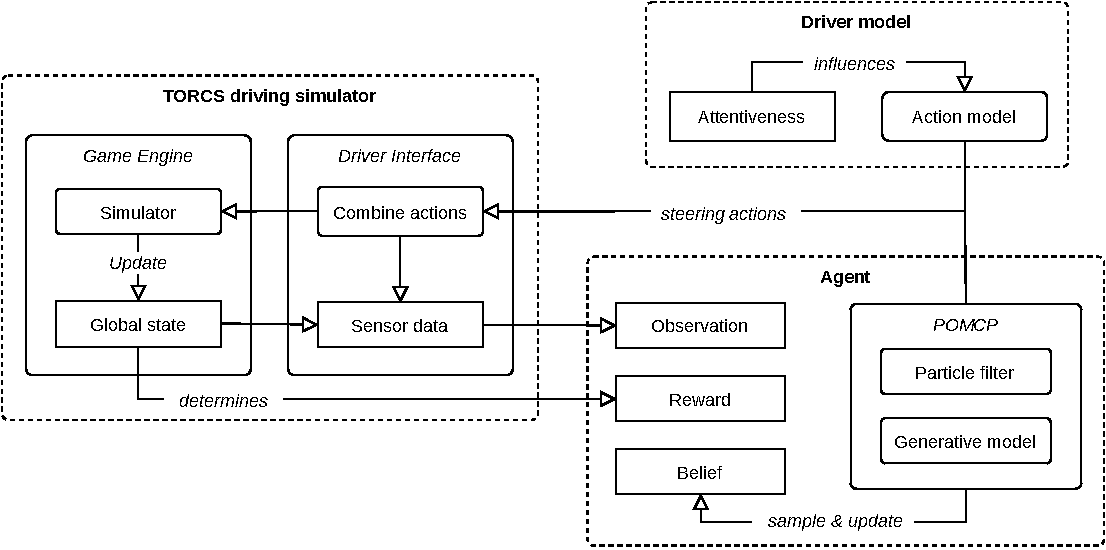
\includegraphics[width=1.0\textwidth]{figures/Components.pdf}
    \caption{Overview of the modules used to represent and solve the shared control lane keeping POMDP}
    \label{fig:overview}
\end{figure}

Rather than experimenting with real humans and a real car, simulation models are is used for both the car and the human driver in experiments. Figure \ref{fig:overview} gives an overview of the three distinct modules employed to represent the problem as a POMDP and solve it: First, the racing car simulator TORCS \parencite{torcs} simulates the dynamics of a car driving on a highway. Second, the driver model substitutes the human driver. Third, the agent applies POMCP in order to solve the POMDP online. The modules are described in detail in the following sections. 

% TODO: Add: The agent can only recognize a state change of the driver after the driver has performed the first action in this state. This is because there are no observable clues about the duration of the driver's attentiveness and distraction.

\subsection{TORCS as a highway driving simulator}
\label{torcs}

\glsentryfull{torcs} is an open-source car driving simulator \parencite{torcs}. As the name suggests, TORCS was initially developed to simulate racing car tournaments. However, as racing cars are fundamentally also just cars and everything, including the tracks, is highly customizable, highway driving can be simulated just as well. Part of TORCS is a comprehensive and realistic discrete-time simulation engine to simulate car dynamics, as well as an \glsentryshort{api} for computer-controlled drivers, so-called robots.

TORCS is used for two purposes in this thesis. First, its simulation engine serves as the environment for the agent and driver. The steering actions of the agent and driver are combined in a TORCS \emph{robot} satisfying the driver interface. TORCS maintains the car's true state and updates it based on the combined steering action. Second, the simulation engine is used as a generative model to sample state and observation transisitions for the forward search performed during the agent's online MCTS policy computation.  
 
 
% TODO: Move this to the next chapter?
\begin{figure}[htbp]
    \centerfloat
    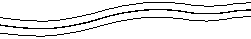
\includegraphics[width=1.0\textwidth]{figures/track.pdf}
    \caption{Course of the road of a section of the TORCS highway track used for experiments.}
    \label{fig:track}
\end{figure}

Typical racing tracks for TORCS have sharp road bends and a generally wide road which can have different widths in its course. This does not reflect a highway driving scenario well. Therefore, a custom highway track is used instead (see Figure \ref{fig:track}). The custom track only has moderate road bends and a constant lane width of 3.75m, as it is common in Europe \parencite{lane_width}. The road is completely flat and there are no other cars on it. Moreover, a fixed speed of 80 kp/h is set during experiments.

\subsubsection{Car state and its updates}
\label{sec:state}

TORCS data model for the car state is too extensive to list here in full\footnote{See tCar struct in the \href{https://sourceforge.net/projects/torcs/files/api-docs/}{TORCS API documentation}}. Most important are the car's position on the track, its current velocity and its accelleration. Among others, there are additional attributes for the state of transmission and engine, the friction and spin of the wheels, and aerodynamic influences such as the current air speed. The values in the state are continuous. Since the problem is a lane keeping task, any state representing a lane departure is consiered a \emph{terminal state}, resulting in the end of an experiment. The car is considered to have departed from its lane if the center of car lies more than 20cm beyond side lane markings.

The state is updated by the simulation engine every 0.002 seconds of simulated time (this is the driving time that is simulated, not real time). By default, robots provide new control actions to the car every 0.02 seconds. However, for the experiments in this thesis, a rate of 0.1 seconds is chosen. This makes the ride less smooth but reduces the frequency in which the agent has to plan ahead, reducing the amount of planning time. The steering action is repeated until a new one is provided.

\subsubsection{Actions}
\label{sec:actions}

Accelleration, braking, and gear changes are performed by a simple controller intended to keep the speed constant at at all times. The human driver and the agent share control of the steering wheel. The steering input of the driver $a_{driver}$ and agent $a_{agent}$ are added to $a_{car} \in [-1, +1]$ using Equation~\ref{eq:steering}. A steering action of $-1$ means steering fully to the right (159 degrees), and an action of $+1$ has the effect of fully steering to the left (21 degrees). 

\begin{equation}
    a_{car} = \min(\, -1, \, \max(\, 1, \, (a_{driver} + a_{agent})\,)\,)
    \label{eq:steering}
\end{equation}

% This is not true. The driver's actions are discretized. This is not having full control. Very important to mark at the driver model
% TODO: Move discretization to driver.pospos fa
% The driver has the  full natural steering control with $a_{driver} \in [-1, +1]$. 

Table \ref{tab:actions} shows the discrete actions for the driver and the agent. The discrete values have been chosen empirically. More actions allow for a more precise control. However, the number of actions is the branching factor for the search tree the agent constructs to solve the POMDP, and thus has a big impact on the complexity of the search problem. Therefore, a compromise between precision and performance is made. Because minor actions are more likely and generally preferable in a highway driving scenario, the resolution is higher for small steering actions.

\begin{table}[htbp]
\footnotesize
\centering
\centerfloat
\setlength{\tabcolsep}{5pt}
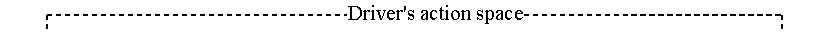
\includegraphics[width=0.925\textwidth]{figures/driver-actions.pdf}
\begin{tabular}{cccccccccccccccc}
\toprule
 -2 & -1     & -0.75  & -0.5   & -0.25  & -0.15  & -0.1   & 0     & 0.1   & 0.15  & 0.25  & 0.5   & 0.75  & 1 & 2 \\ \bottomrule
\end{tabular}
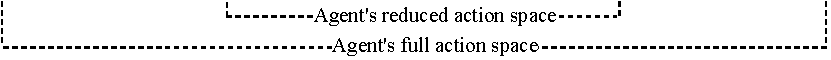
\includegraphics[width=0.925\textwidth]{figures/agent-actions.pdf}
\caption[Discrete steering actions for the driver and the agent]{Discrete steering actions for the driver and the agent.}
\label{tab:actions}
\end{table} 

If the driver is distracted while the car is in a road bend, in the most extreme situation, she could potentially steer into the opposite direction of where she needs to steer in oder to keep the car centered in its lane. In this case, to correct the driver's incorrect action, the agent needs to be able to effectively reverse the driver's action. Therefore, the action space of the agent is extended by plus two and minus two. The agent is evaluated in experiments with the full action set but also with a small subset of the full action set including only minor actions (reduced action space in Table \ref{tab:actions}).

\subsubsection{Observations}
\label{sec:observations}

In a POMDP, the agent has only partial information about the true state of the environment. The information the agent has stems from observations it makes by interacting with the environment. For the shared control lane keeping task, the agent is given an observation after every steering action (after every 0.1 seconds of simulated time). It observes the current horizontal position of the car (lane centeredness), the car's relative yaw angle with respect to the track axis, and the driver's action from the last time step. The driver's current steering action is not observable. The agent has to estimate the most likely next action of the driver by considering the history of past observations. 

\begin{figure}[htbp]
    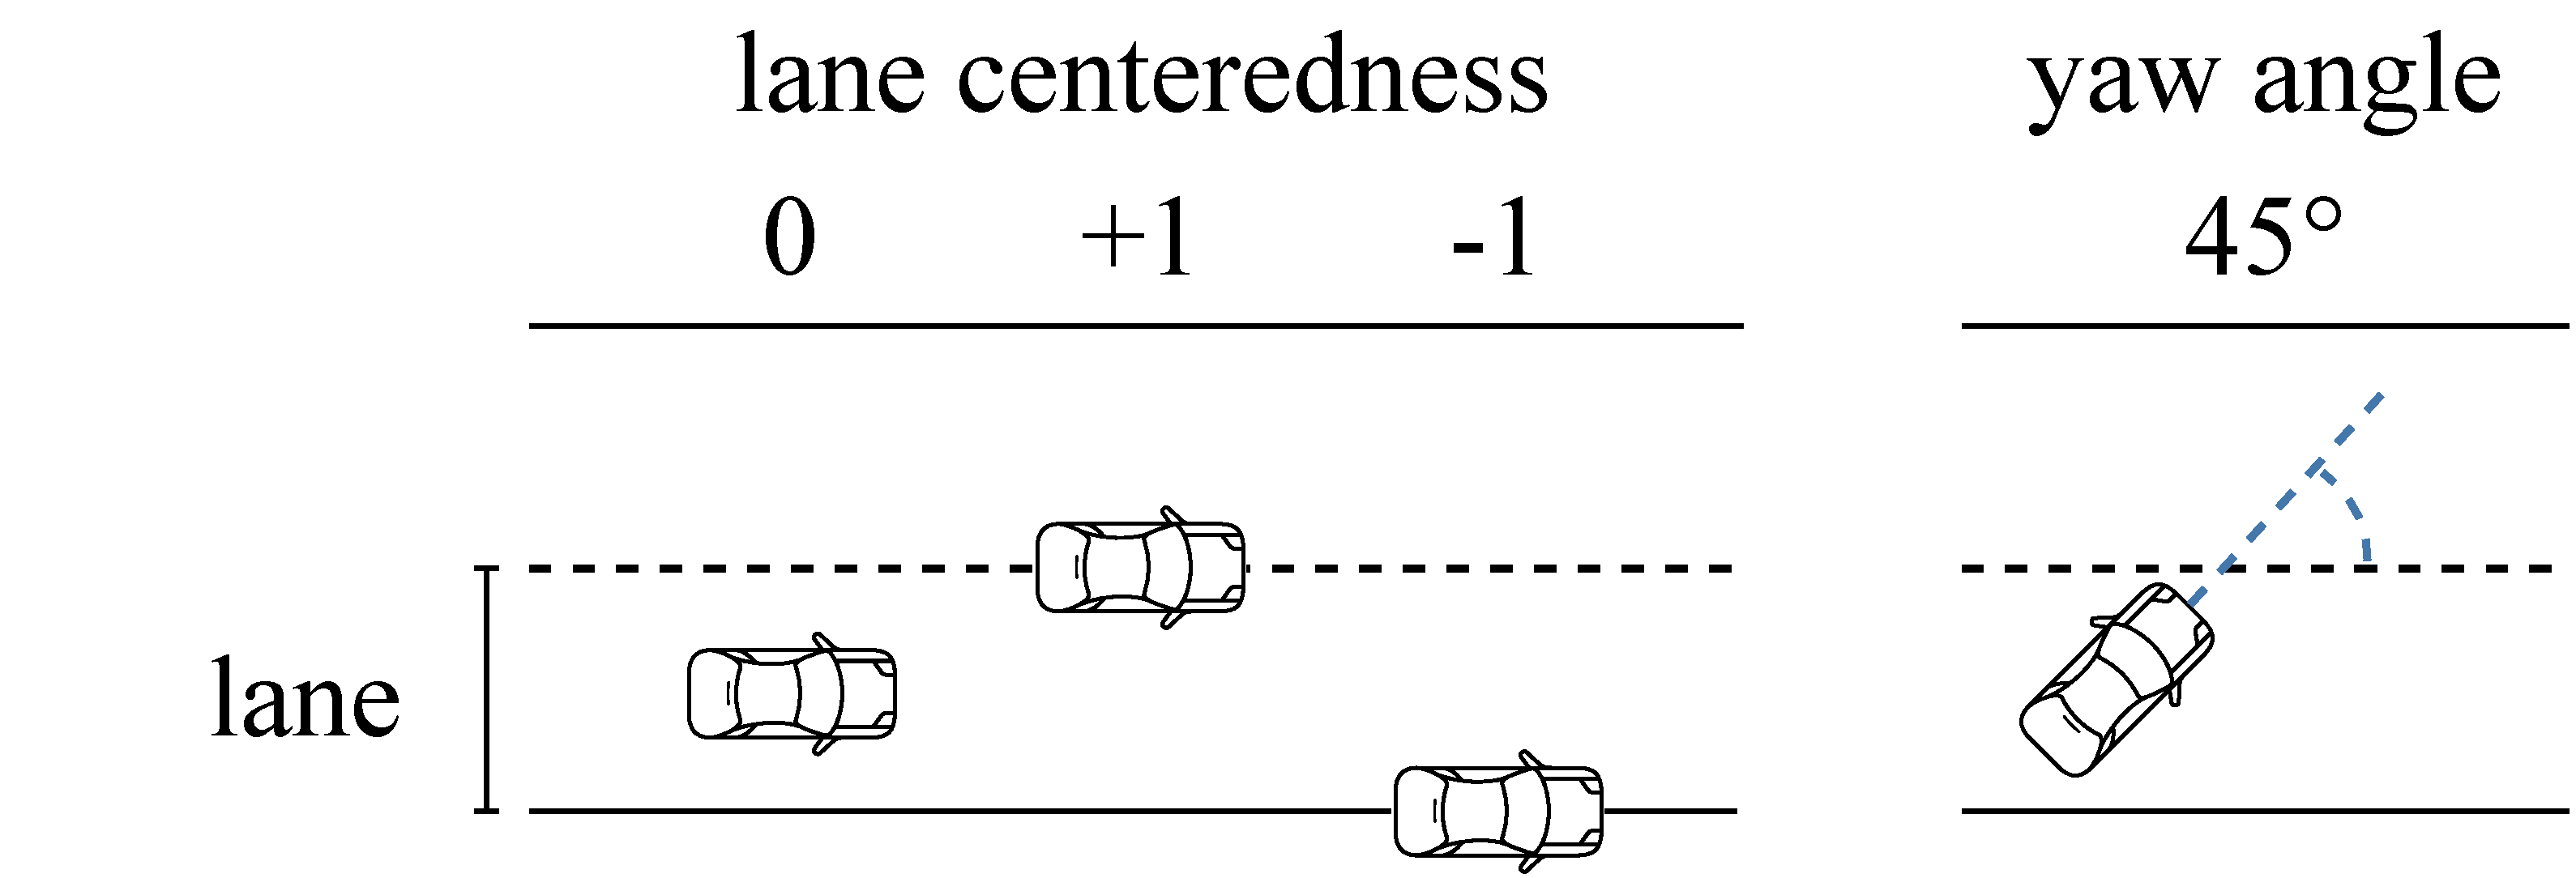
\includegraphics[width=0.6\linewidth]{figures/angle_distance.pdf}
    \centering
    \caption{Illustration of lane centeredness and yaw angle values}
    \label{fig:observations}
\end{figure}

The observations are discrete. The lane centeredness is originally in a continuous interval of $(-\infty,\infty)$, with values in between -1 (right lane border) and +1 (left lane border) denoting that the car is within its lane, and everyting beyond standing for an off-track position (see Figure \ref{fig:observations}). 99 discrete values represent evenly spaced segments between -1 and +1, and two additional values stand for left off lane and right off lane positions. The angle is transformed from an interval of $[-\pi, +\pi]$ radians to 101 discrete values representing evenly spaced segments. The driver's action is discretized as stated in the last section.

\subsection{Driver model}
\label{sec:driver_model}

Instead of performing experiments with an actual human driver, the driver is simulated using a stochastic driver model. The driver model determines when a driver is attentive or becomes distracted, for how long the attentive or distracted period persists, and what actions the driver takes. The driver model is rather simple. If the agent can plan successfully with a simple driver model, this serves as an initial confirmation that the solution approach is promising. The focus of this thesis is not a realistic driver model.

% TODO: Add driver model illustration

\subsubsection{Configurations}

Three different driver model configurations with increasingly complex dynamics are used in the experiments:
\begin{enumerate}
    \item \textbf{Simple driver model:} The simplest model steers optimally when the driver is attentive, and if it is in a distracted state, the model repeats the last attentive steering action until the driver regains her attentiveness. A distracted driver's ability to notice changes in the course of the road is limited because of a reduced situational awareness and therefore she does not adjust to road changes like an attentive driver would (\cite{driver-awareness}; \cite{driver-awareness2}).
    \item \textbf{Steering overcorrection:} Another, more complex scenario, is based on the assumption that a driver who has just regained attentiveness after having been distracted performs an overly strong steering correction during her first action, and thereby overshoots. The first action of the attentive driver is increased by a random amount between 10 and 25 percent. The over correction is added to the continuous driver action before discretization.
    \item \textbf{Steering overcorrection and noise:} The last, most complex scenario introduces action noise. It acts just like the second scenario, just with an additional random noise between five and 20 percent. The action can thereby become five to 20 percent stronger or weaker. The noise is intended to make the driver less predictable. It is also added before the action discretization is applied.
\end{enumerate}
\label{sec:driver_act_discr}
The actions of the driver are discretized by mapping their continuous values to the closest vaue in the discrete action space as it can be seen in Table \ref{tab:action_dist}.

\begin{table}[htbp]
\footnotesize
\centering
\centerfloat
\setlength{\tabcolsep}{3pt}
\begin{tabular}{@{}lccccccccccccc@{}}
\toprule
Action & -1     & -0.75  & -0.5   & -0.25  & -0.15  & -0.1   & 0     & 0.1   & 0.15  & 0.25  & 0.5   & 0.75  & 1 \\ \midrule
From   & -1   & -0.875 & -0.625 & -0.375 & -0.2   & -0.125 & -0.05 & 0.05  & 0.125 & 0.2   & 0.375 & 0.625 & 0.875 \\ 
To     & -0.875 & -0.625 & -0.375 & -0.2   & -0.125 & -0.05  & 0.05  & 0.125 & 0.2   & 0.375 & 0.625 & 0.875 & 1  \\ \bottomrule
\end{tabular}

% TODO: Fix caption!
\caption[Driver action discretization]{Driver action discretization. For negative values, the \emph{To} value is exclusive. For zero, both \emph{From} and \emph{To} are inclusive. For positive values, the \emph{From} value is exclusive.}
\label{tab:action_dist}
\end{table} 

\subsubsection{Driver state and its updates}

The driver state consists of two variables: The current state (attentive or distracted), and the duration it remains in its current state. The driver model is initially set to an attentive state. The duration it remains in this state is randomly chosen but lies between one second (10 actions) and 5 seconds (50 actions) of simulated time. Every 0.1 seconds, an action is chosen depending on the driver's current state. Afterwards, the remaining duration is decremented by 0.1. When the time runs out for the curren state, the state reverses; an attentigve driver becomes distracted and a distracted driver regains attentiveness. The duration for the resulting state is randomly chosen again. The process repeats until the experiment is over.

\subsection{Reward}
\label{sec:reward}

The reward function defines the goal of the agent. For the task of lane centering, two sub-goals need to be considered: First, the car is supposed to stay as close to the lane center as possible. Second, the car's yaw angle (the direction into which the car is headed) should be as close to the track axis angle as possible. 

Equation \ref{eq:reward} shows the reward function for the agent that incorporates both targets. The relative yaw angle is denoted as $\theta$, and $\phi$ represents the lane cen0teredness (see Figure \ref{fig:observations}). A lane centerednss of zero means the car is centered. If the car is on the left most side of the lane, the value equals one, for the right most side it equals minus one. The agent receives the maximum reward if the car is in the middle of the road, while its relative yaw angle is equal to zero. Similar reward formulations have been used successfully before (\cite{reward1}; \cite{reward2}). The attentiveness of the driver is not directly included in the reward function. However, it is implicitly considered. If the agent performs an action that leads to a suboptimal combined steering action, it is penalized by receiving a lower reward. Thereby, if the agent acts when the attentive driver behaves optimally, it is punished indirecly.

\begin{equation}
    \label{eq:reward}
    R = 
    \begin{cases}
        \cos \theta + |\phi|,& \text{if } \phi \in [-1,+1]\\
        0,              & \text{otherwise}
    \end{cases}
\end{equation}

\section{Solution approach using the POMCP algorithm}

\subsection{General POMCP definition}
\label{sec:pomcp}

% explain: 
% - Planning versus learning
% - How POMCP breaks the curse of dimensionality with Monte-Carlo sampling
% - Belief and blief update

% Particle filter belief update:
% See (POMDP, Thesis) Tactical Decision-Making forHighway Driving

% TODO: Mark rollout and search phase as in the original paper

\begin{figure}[htbp]
    \centering
    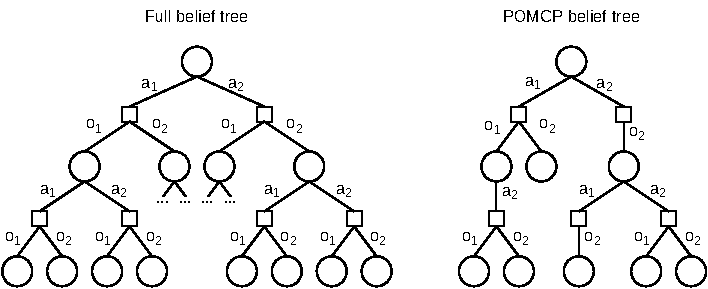
\includegraphics[width=0.8\textwidth]{figures/pomcp_belief_tree.pdf}
    \caption[A full belief tree in contrast with a POMCP belief tree]{Contrasting a full belief tree (left) with a POMCP belief tree (right) for a POMDP with two actions and two observations and a time horizon of two. A belief is stored at every circle node. The full belief tree has 21 belief nodes, while the POMCP belief tree has just nine. The number of nodes of the full belief tree grows exponentially with the time horizon (curse of history), whereas the POMCP belief tree only contains a number trajectories which have been sampled from a generative model. By performing the sampling, the size of the tree is reduced and the curse is \textit{broken}.}
    \label{fig:full_vs_pomcp}
\end{figure}
% TODO: Illustrate belief tree
% See Figure 1 in DESPOT

The key idea of \Gls{pomcp} is to use Monte Carlo sampling both to sample start states from the belief and to sample histories using a generative model \parencite{pomcp}. 

The number of histories to consider in a POMDP grows exponentially with respect to the depth of the planning horizon. This is called the curse of history. POMCP overcomes this limitation by using a generative model to sample state transitions. By doing so, only a subset of histories is considered; the size of the belief tree is reduced and the curse is \textit{broken} (see Figure \ref{fig:full_vs_pomcp}). Furthermore, there is the curse of dimensionality. The belief space has the same dimensionality as the number of states. Thus, the number of beliefs to consider grows exponentially with the number of states. POMCP uses the states encountered during the construction of the tree to represent the belief. Start belief states are sampled from these states, effectively limiting the number of considered belief states and thereby also breaking the second curse. 

POMCP constructs a search tree representing histories $h$ of actions and observations. At each node, $N(h)$ stores the number of times the node and thereby the coresponding history $h$ has been visited during the sampled trajectories simulated with the generative model. $V(ha)$ gives the action node's expected value that is approximated by the average return of simulations starting at history $h$ and performing action $a$. At every observation node, the belief over the states is maintained by employing a particle filter. Each observation node stores a collection of all states that led to the represented observation during planning. Whenever an observation occurs, the corresponding state is stored in this collection. The states in the collection are called particles and together the particles represent the agent's belief B(h) at the corresponding observation node. The more likely a belief state is, the more often it occurs as a particle in the belief. By using the particle filter method, expensive belief update calculations are not necessary. The collection of states alone aproximates the posterior probability distribution for the belief.

\begin{figure}[htbp]
    \centerfloat
    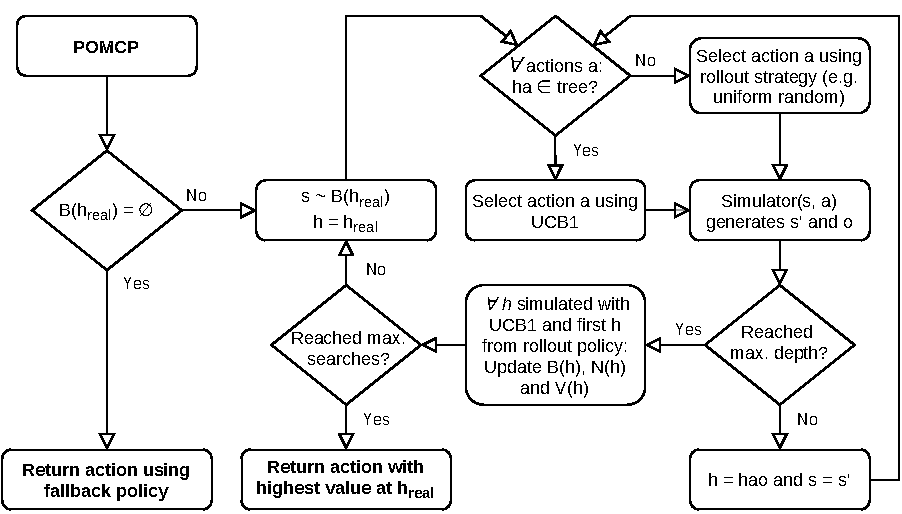
\includegraphics[width=1.0\textwidth]{figures/POMCP.pdf}
    \caption{Flow chart illustrating the \glsentryfull{pomcp} algorithm}
    \label{fig:pomcp}
\end{figure}

Figure \ref{fig:pomcp} illustrates the process of POMCP. The algorithm starts with an initial belief about the environment. If the belief for the current history $h_{real}$ does not contain particles in the beginning of a planning episode, the agent has lost track of the environment's state completely. One could construct a new belief by sampling the state space in this case. However, for the car driving scenario, this approach is too inaccurate. Accessing the real state of the environment to build the belief would be cheating. Instead, we consider the planner to have failed and select actions randomly from this point on.

To select which action to perform in the real environment, a fixed number of forward searches is performed from the current history (often a certain maximum planning time is used alternatively). During these searches using the generative model, the belief and the expected action values are updated. After all searches are complete, the action $a_{best}$ with the highest value at the current history $h_{real}$ is returned. After this action is executed in the real environment, with an observation $o_{last}$ the tree can be pruned. Only the nodes from history $h_{real}a_{best}o_{last}$ onward stay relevant as all other histories are rendered impossible. Then, the process repeats from the new history.

The start state for each search is sampled from the belief at the curret history. The search tree is searched in two stages: Simulation and rollout. As long as the search tree contains child nodes for all actions at the currently considered history, the simulation stage is active. During the simulation stage, no new nodes are added to the tree. The tree is searched using the \glsentryfull{ucb1} algorithm to select actions \parencite{ucb1}. UCB1 chooses actions by the principle of optimism in the face of uncertainty. Even with just little knowledge, the algorithm selects the best action greedily. If this optimistic guess turns out to be correct, the algorithm can further continue to exploit this action and regret is+ kept to a minimum. If the action leads to a bad return, its value is assumed to deteriorate quickly, allowing the algorithm to select an alternative action. Exploration is controled by enhancing the value of rarely-tried actions with a fixed exploration bonus. 

State transitions are simulated using the generative model. Given the current history and chosen action, the generative model returns a successive state $s'$, observation $o$, and reward $r$. The successive state $s'$ is then added to the belief at the observation node corresponding to $o$ and the count for the current history is incremented. The search continues from $s'$ in the same manner. 

If any history is visited for the first time during the simulation stage, the algorithm continues in the rollout stage. First, all action nodes are initialized with initial counts an values. These are usually 0, unless preferred actions are used (See Section \ref{sec:preferred_actions}). Then, the history is \textit{rolled out} further using uniform random action selection and the generative model. The process is continually repeated using the succeeding states from the generative model until a maximum depth is reached in the tree. During the rollout, no further nodes than the ones just initialized are added to the tree. The tree's growth is thereby limited to one level of depth per search. The main purpose of the rollout is to form a first estimation of the newly encountered history. After every search, the values at all nodes encoutered during the search are updated by backpropagating the rewards through the tree.

\subsection{Action and observation space discretization}
\label{sec:discretization}

POMCP is not intended to be used to solve continuous POMDP. However, using POMCP with a continuous states is possible as the particle filter approach can still provide a good approximation of the belief as long as the number of samples is large enough. To account for continuous action and observation spaces, discretization is necessary. Figure \ref{fig:pomcp_cont} shows how POMCP behaves when tasked with solving POMDP with continuous observation or acrtion spaces. If the observations are continuous, the search tree cannot extend beyond the first observation layer as most likely, every observation is unique and thus, no history will ever be visited twice. In the case of continuous actions, the chance of exectuing the same exact action twice is very low. Therefore, in this case likewise no history is reached twice. Planning becomes impossible. However, POMCP can be successfully applied with continuous POMDP by discretizing the action and observation spaces \parencite{pomcp_continuous}.

\begin{figure}[htbp]
    \centering
    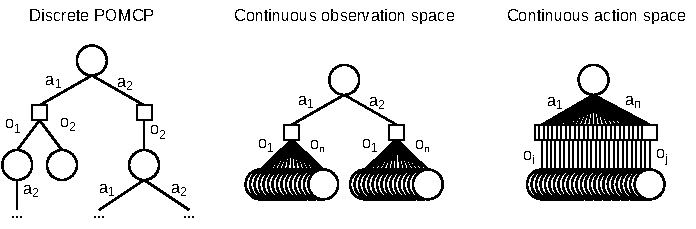
\includegraphics[width=1.0\textwidth]{figures/pomcp_continuous.pdf}
    \caption[Comparison of POMCP belief trees with discrete observations and continuous observations]{Comparison of POMCP belief trees with discrete observations (left) and continuous observations (right) with two actions.}
    \label{fig:pomcp_cont}
\end{figure}

The action space is discretized as outlined before in Section \ref{sec:actions} and the discretization of the observation space is defined in Section \ref{sec:observations}. A balanced discretization resolution is chosen empirically. A too fine grained discretization leads to very wide belief trees and can thereby hinder convergence, while a coarse discretization increases the convergence probability but comes with a lower precision in planning.


% TODO: Add actions and observations tables

\subsection{Particle deprivation and particle injection}
\label{sec:particle_deprivation}

Particle filter approaches, POMCP included, can fail due to a phenomenon called particle deprivation. Because of the random nature of the process, the belief can sometimes converge towards a state that is far from the environment's true state. Particles that differ from the converged state have a low probability to be selected while sampling (low relative count). Hence, with each iteration, they become scarcer until they are completely erased from the belief. At this point, the agent is sure to be in an erroreous state and cannot recover anymore. Particle injection (also called particle reinvigoration) is a method to counteract this problem by introducing a number of random particles to the belief at each iteration \parencite{decision_making_book}. While this reduces the accuracy of the belief, it prevents its complete convergence towards a wrong state. 

Particle injection is used to increase the variance of the belief about the driver model state. Only observable information is used. Concretely, particle injection is implemented by adding driver model states with a random number of remaining actions and the same action as the one that was last observed. The number of remaining actions can be lower than the minimum defined in Section~\ref{sec:driver_model} because this limit is only intended for initial sampling and the true remaining number of driver actions in a particular state might be lower after having performed actions already. Like in the original POMCP paper, the amount of transformed particles that are added before each planning step is $1/16$ of the number of searches. The particles can be added during policy execution, and therefore, do not influence planning time.

% Use term posterior probability distribution? We can only add particles after making an observation so that we can verify that the potential particles to add match this belief.


\subsection{Preferred actions}
\label{sec:preferred_actions}

Preferred actions are a way to pass domain knowledge to the agent. In the case of the lane keeping scenario on a highway, one thing to consider is that strong steering actions are seldomly needed. Strong actions should only be needed as countermeasure when a distracted driver turns significantly into the wrong direction. 

% TODO: Just say the agent does not act anymore when losing track with the belief instead of using uniformly random action selection? Makes more sense.

% This is strongly related to the particle deprivation problem described in Section~\ref{sec:particle_deprivation}. When the driver is in a distracted or attentive state, any number of remaining actions in this state below the maximum number (see Section~\ref{sec:driver_model}) could be valid and can therefore be part of the driver model states in the belief. In successive iterations, particles that represent drivers switching their state earlier than the true driver, and therefore change their steering behavior, are ruled out and removed from the belief. Thereby, after some iterations, driver model states that have the same or more remaining actions than the true state dominate the belief.

% preferred actions = domain knowledge

\subsection{Generative model}
\label{sec:gen_model}

